%=====================================================
% Sections/03-CoSoLyThuyet.tex
% Chương 3 -- Cơ sở lý thuyết
%=====================================================

\section{Cơ sở lý thuyết}

Chương này trình bày các khái niệm và nguyên lý trực tiếp phục vụ việc xây dựng trợ lý
mua sắm đa phương thức. Phần công nghệ cụ thể, cấu hình triển khai và mã nguồn được
trình bày ở các chương sau; vì vậy nội dung dưới đây tập trung vào mô hình hóa bài toán,
cơ chế xử lý và cơ sở đánh giá.

\subsection{Tìm kiếm sản phẩm đa phương thức}

Tìm kiếm đa phương thức cho phép người dùng cung cấp văn bản, hình ảnh hoặc đồng thời
cả hai loại dữ liệu; dạng tương tác kết hợp văn bản và hình ảnh thường được gọi là
multisearch \parencite{google2022multisearch}. Với truy vấn văn bản, hệ thống phân tích
nhu cầu và các thuộc tính như danh mục, màu sắc, kích thước và khoảng giá. Với truy vấn
hình ảnh, hệ thống biểu diễn đặc trưng thị giác rồi tìm các sản phẩm có hình dạng, màu
sắc hoặc kiểu dáng tương tự. Truy vấn kết hợp dùng hình ảnh để mô tả kiểu dáng và văn
bản để bổ sung điều kiện nghiệp vụ, chẳng hạn ``mẫu tương tự nhưng màu đen, dưới một
triệu''.

Tìm kiếm dựa hoàn toàn trên từ khóa chỉ nhận biết sự trùng khớp bề mặt nên dễ bỏ sót
đồng nghĩa, lỗi chính tả, cách viết không dấu và các cách diễn đạt khác nhau. Tìm kiếm
ngữ nghĩa khắc phục hạn chế này bằng cách so sánh biểu diễn của truy vấn và sản phẩm,
sau đó xếp hạng các ứng viên theo mức độ liên quan. Trong trợ lý mua sắm, kết quả tìm
kiếm còn phải liên kết với giỏ hàng, đơn COD và dữ liệu tồn kho; giá, tồn kho và trạng
thái đơn luôn phải được Backend kiểm chứng.

Trong trợ lý mua sắm, tìm kiếm chỉ là một bước của chuỗi tương tác. Hệ thống còn phải
giải thích lựa chọn, hỏi lại khi thiếu thông tin và duy trì tiêu chí qua nhiều lượt. Do đó,
kết quả AI không được
tự xem là nguồn dữ liệu giao dịch; giá, tồn kho và trạng thái đơn phải được kiểm chứng
bởi Backend.

\subsection{Embedding và không gian ngữ nghĩa}

Embedding là phép ánh xạ một đối tượng thành vector số thực có số chiều cố định. Với
văn bản, SBERT sử dụng mạng siamese/triplet để tạo sentence embedding có thể so sánh
bằng cosine similarity \parencite{sbert2019sentence}. Trong bài toán sản phẩm, text
embedding có thể được tạo từ tên, mô tả, danh mục và thuộc tính; image embedding giữ
các đặc trưng thị giác như hình dạng, màu sắc, họa tiết và chất liệu biểu kiến.

Các mô hình thị giác--ngôn ngữ như CLIP dùng hai encoder và mục tiêu học tương phản để
đưa văn bản và hình ảnh phù hợp vào gần nhau trong một không gian biểu diễn chung
\parencite{clip_paper}. Cách biểu diễn này cho phép truy hồi trực tiếp từ một modality
sang modality còn lại, nhưng không phải mọi hệ thống đa phương thức đều sử dụng chung
một không gian vector.

\begin{figure}[H]
    \centering
    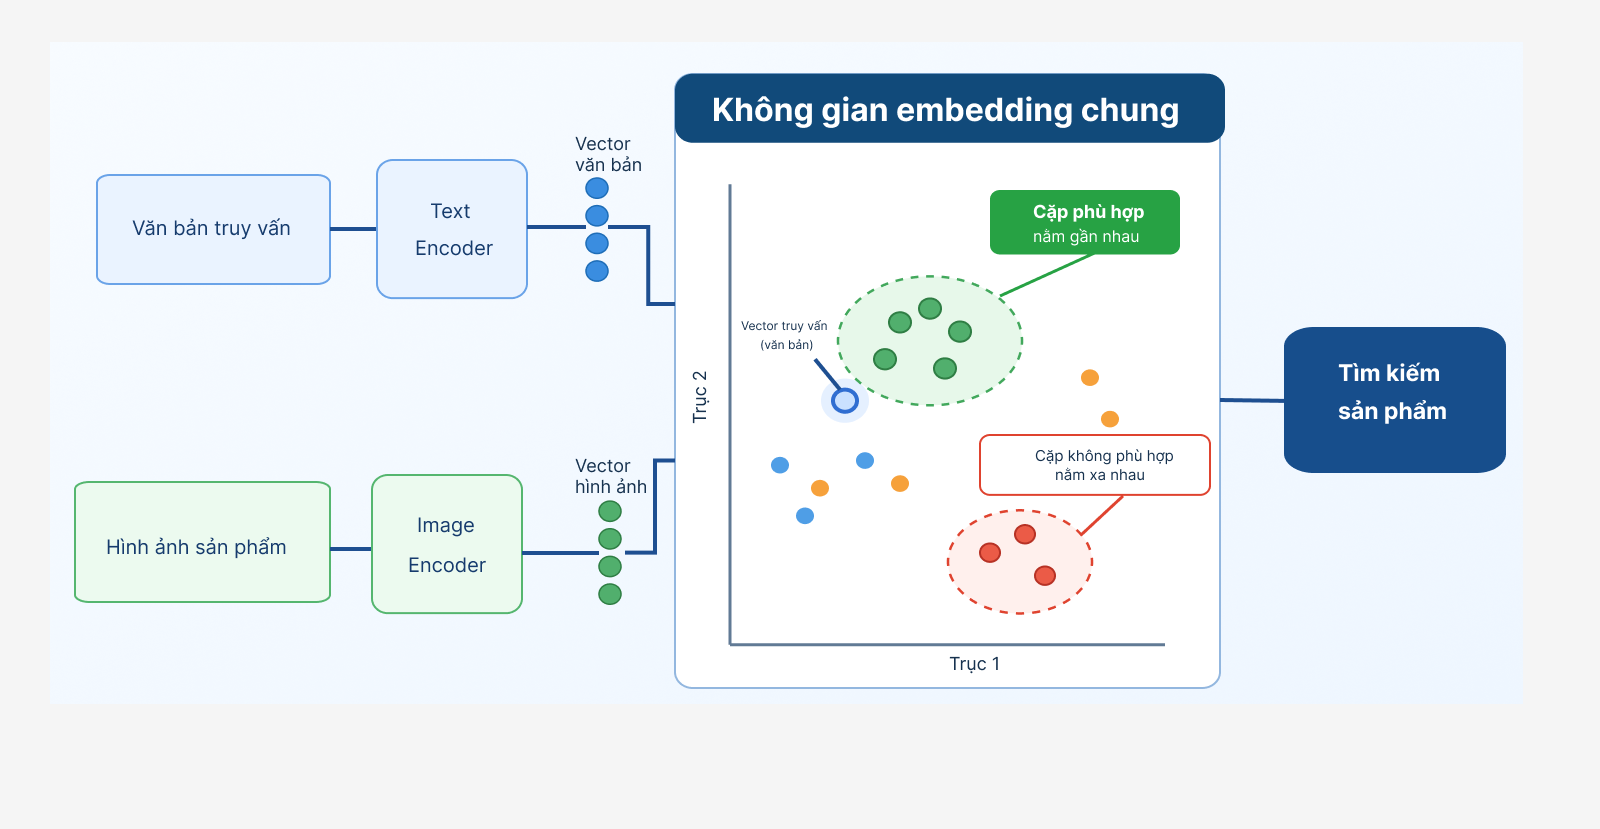
\includegraphics[width=0.84\textwidth]{Images/Cosolythuyet/Ánh xạ văn bản và hình ảnh vào không gian embedding chung để truy hồi đa phương thức.png}
    \caption{Ánh xạ văn bản và hình ảnh vào không gian embedding chung để truy hồi đa phương thức (ảnh thực hiện bằng Figma)}
    \label{fig:shared_embedding_space}
\end{figure}

Hình~\ref{fig:shared_embedding_space} minh họa hai encoder tạo ra vector cho truy vấn
văn bản và ảnh sản phẩm. Trong không gian chung, các cặp phù hợp nằm gần nhau; các cặp
không phù hợp nằm xa nhau. Đây là nguyên lý chung của truy hồi đa phương thức dùng
không gian biểu diễn chung. Trong đề tài, Text Search thực hiện text-to-text retrieval,
Image Search thực hiện image-to-image retrieval, hai loại embedding được lưu trong các
collection riêng và không được cộng hoặc so sánh trực tiếp. Mã sản phẩm và metadata
liên kết kết quả giữa các collection; các điều kiện chính xác như giá tối đa hoặc trạng
thái đang bán vẫn phải được kiểm tra riêng.

% Embedding không thay thế bộ lọc thuộc tính. Vector có thể nhận ra ``đầm dự tiệc'' gần
% với ``váy mặc sự kiện'', nhưng không bảo đảm điều kiện giá tối đa hoặc trạng thái còn
% bán. Các điều kiện chính xác phải được lưu dưới dạng metadata và kiểm tra ở bước lọc.

% Trước khi truy hồi, vector thường được chuẩn hóa $L_2$ để loại ảnh hưởng của độ lớn:
% \begin{equation}
%     \widehat{\mathbf z}=\frac{\mathbf z}{\lVert\mathbf z\rVert_2},
%     \qquad
%     s(\mathbf z_t,\mathbf z_i)=\widehat{\mathbf z}_t^{\mathsf T}\widehat{\mathbf z}_i.
%     \label{eq:embedding_normalization}
% \end{equation}
% Trong huấn luyện tương phản, một cặp văn bản--ảnh đúng được kéo lại gần và các cặp
% khác trong cùng minibatch được đẩy ra xa. Với nhiệt độ $\tau$ và batch $B$, một dạng
% InfoNCE cho một truy vấn văn bản là
% \begin{equation}
%     \mathcal{L}_{\mathrm{NCE}}=-\log
%     \frac{\exp\!\left(s(\mathbf z_t,\mathbf z_i)/\tau\right)}
%     {\sum_{j=1}^{B}\exp\!\left(s(\mathbf z_t,\mathbf z_j)/\tau\right)}.
%     \label{eq:infonce_loss}
% \end{equation}
% Mục tiêu này giải thích vì sao hai encoder có thể hỗ trợ truy hồi chéo modality, nhưng
% không thay thế việc kiểm tra mã sản phẩm và thuộc tính nghiệp vụ.

\subsection{Truy hồi vector và Approximate Nearest Neighbor}

Cơ sở dữ liệu vector lưu mỗi điểm gồm định danh, vector và payload metadata. Payload của
sản phẩm có thể chứa mã sản phẩm, danh mục, thương hiệu, màu, giá và trạng thái kinh
doanh; nhờ đó similarity search có thể kết hợp với metadata filtering trong các hệ
quản trị vector như Milvus và Qdrant \parencite{wang2021milvus,qdrant2024vectorsimilarity}.

Với hai vector $\mathbf q$ và $\mathbf x$, cosine similarity được xác định bởi
\begin{equation}
    \operatorname{cos}(\mathbf q,\mathbf x)=
    \frac{\mathbf q\cdot\mathbf x}
    {\lVert\mathbf q\rVert_2\lVert\mathbf x\rVert_2}.
    \label{eq:cosine_similarity}
\end{equation}
Cosine phù hợp khi hướng vector quan trọng hơn độ lớn; Euclidean distance đo khoảng cách
trực tiếp giữa hai điểm. Việc chọn metric phải nhất quán với mô hình embedding và cách
chuẩn hóa vector.

Với hai vector trong không gian $d$ chiều, khoảng cách Euclidean được tính bởi
\begin{equation}
    d(\mathbf q,\mathbf x)=
    \sqrt{\sum_{j=1}^{d}(q_j-x_j)^2}.
    \label{eq:euclidean_distance}
\end{equation}
Giá trị càng nhỏ thể hiện hai vector càng gần nhau theo metric này, trong khi cosine
chỉ xét góc giữa hai vector. Hệ thống phải dùng cùng metric khi lập chỉ mục và khi truy vấn.

Khi số lượng vector lớn, duyệt toàn bộ dữ liệu có chi phí tuyến tính. Approximate Nearest
Neighbor (ANN) tìm một tập lân cận gần đúng để giảm độ trễ, chấp nhận đánh đổi nhỏ về
độ chính xác. HNSW tổ chức các liên kết thành nhiều tầng:
tầng trên giúp nhảy nhanh giữa các vùng xa, tầng dưới tinh chỉnh các láng giềng gần
\parencite{arya1998optimal,malkov2018efficient}.

Hình~\ref{fig:hnsw_overview} minh họa đường đi từ điểm vào ở tầng cao xuống các láng
giềng gần nhất ở tầng thấp trong quá trình truy hồi.

\begin{figure}[H]
    \centering
    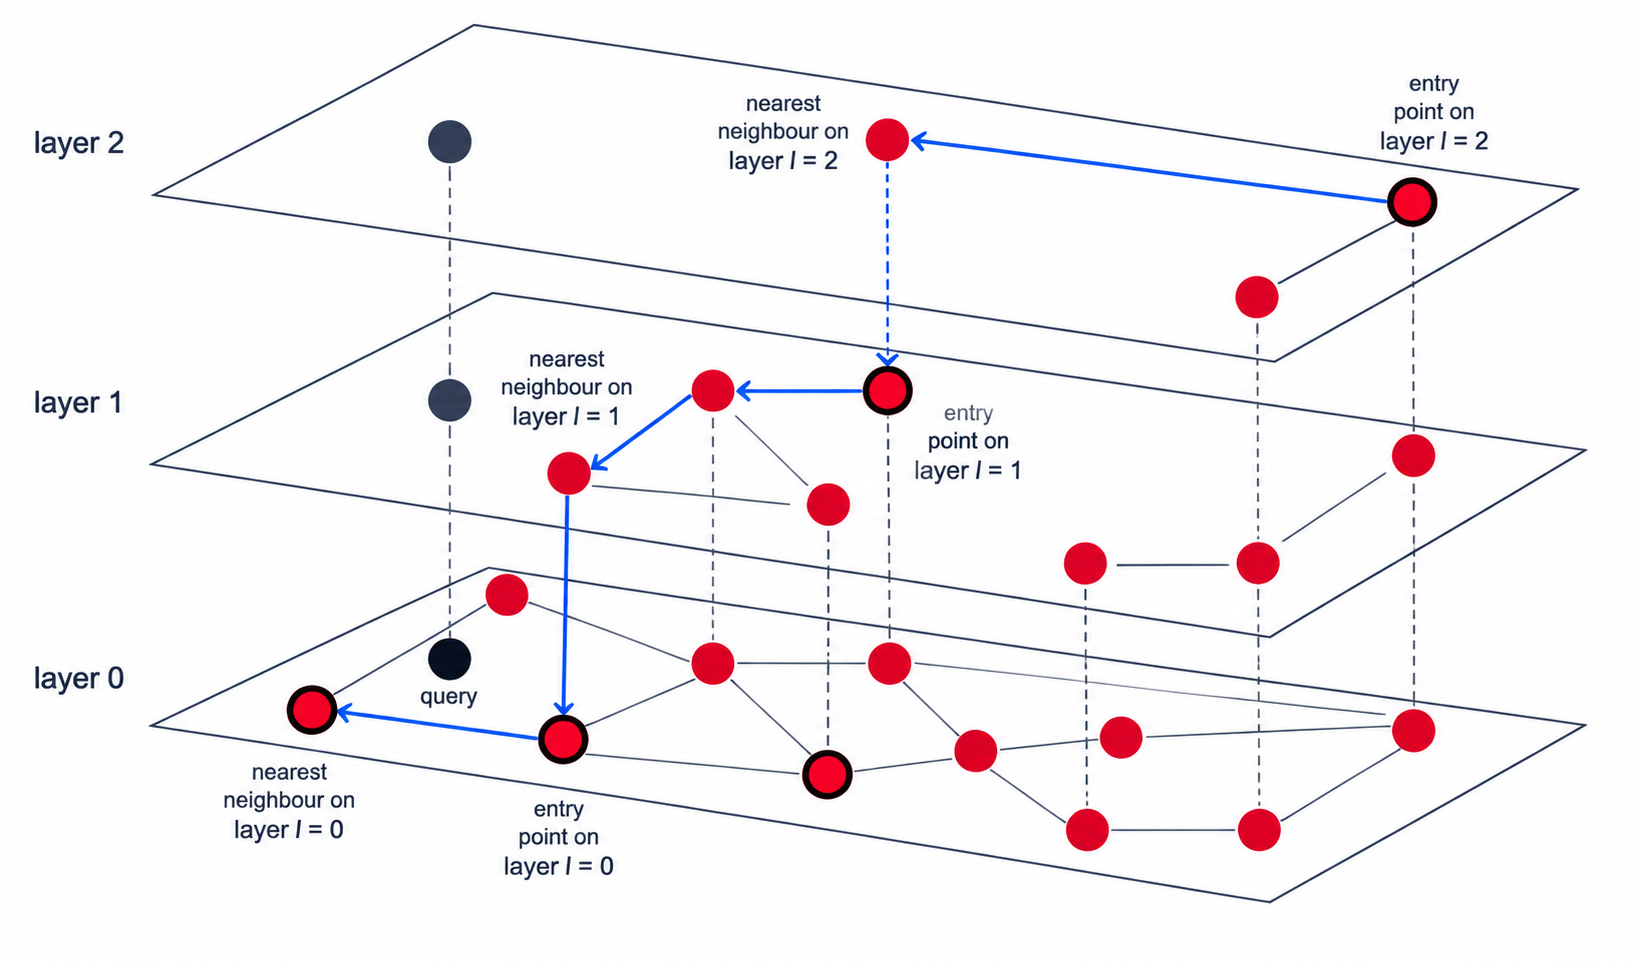
\includegraphics[width=0.78\textwidth]{Images/Cosolythuyet/hnsw-overview.png}
    \caption{Minh họa đồ thị nhiều tầng HNSW cho tìm kiếm lân cận gần đúng
    \parencite{qdrant2024hnsw}}
    \label{fig:hnsw_overview}
\end{figure}

Trong triển khai HNSW, $M$ điều khiển số liên kết tối đa của mỗi nút, còn
$efConstruction$ ảnh hưởng chất lượng đồ thị khi lập chỉ mục và $efSearch$ điều khiển
kích thước hàng đợi ứng viên khi truy vấn. Tăng các tham số này thường cải thiện recall
nhưng làm tăng bộ nhớ, thời gian xây dựng hoặc độ trễ; vì vậy cần chọn chúng bằng
benchmark trên cùng tập truy vấn và cùng metric.

\subsection{Phân tích truy vấn và lọc thuộc tính}

Query understanding xác định ý định và trích xuất các trường có cấu trúc từ phát biểu
của người dùng \parencite{li2010queryunderstanding}. Các ý định chính gồm tìm kiếm văn bản, tìm kiếm
ảnh, tìm kiếm kết hợp, hỏi thông tin, so sánh, làm rõ và tiếp tục hội thoại. Kết quả
có thể được biểu diễn bằng JSON gồm \texttt{intent}, \texttt{query}, \texttt{category},
\texttt{color}, \texttt{size} và \texttt{price\_range}, giúp các bước sau kiểm tra được
dữ liệu thay vì phụ thuộc vào chuỗi tự do.

Chuẩn hóa đưa truy vấn có dấu/không dấu, tiếng Việt/tiếng Anh, viết tắt và lỗi gõ về
dạng nhất quán. Bảng bí danh ánh xạ các tên gọi tương đương vào danh mục và thuộc tính
chuẩn. Query rewrite bổ sung ngữ cảnh còn hiệu lực trong hội thoại nhưng không được tự
ý tạo ra ràng buộc mà người dùng chưa nêu.

Ràng buộc cứng, như giá tối đa, thương hiệu được chỉ rõ hoặc sản phẩm đang bán, được
dùng để loại ứng viên không hợp lệ. Ràng buộc mềm, như phong cách hoặc sắc độ màu suy
diễn, được dùng để cộng điểm thay vì loại bỏ tuyệt đối. Cách phân biệt này giữ được
precision cho yêu cầu bắt buộc mà vẫn duy trì recall khi metadata chưa đầy đủ.

\subsection{Hybrid Search theo chính sách image-conditioned}

Trong đề tài, Hybrid Search là truy vấn đồng thời chứa ảnh tham chiếu và văn bản mô tả
yêu cầu mới; thuật ngữ ``hybrid'' chỉ loại đầu vào, không đồng nghĩa với fusion điểm.
Ảnh được dùng để xác định nhận dạng và độ tương tự trực quan; văn bản được chuẩn hóa
thành các ràng buộc bắt buộc, thuộc tính ưu tiên hoặc điều kiện loại trừ. Các ràng buộc
bắt buộc được áp dụng như bộ lọc để loại ứng viên không hợp lệ, thay vì chỉ trừ điểm.

Nếu số ứng viên hợp lệ chưa đủ Top-$k$ hoặc tín hiệu ảnh yếu, hệ thống mới truy hồi text
collection để tìm thêm mã sản phẩm. Các ứng viên phục hồi vẫn phải vượt toàn bộ ràng
buộc và được chấm lại trên image collection. Vì vậy, nhánh văn bản chỉ mở rộng candidate
pool, không cung cấp điểm để fusion với điểm ảnh.

Với ứng viên hợp lệ, hệ thống sắp xếp giảm dần theo điểm cosine do image collection trả
về. Khi người dùng truyền rõ màu hoặc danh mục, một mức boost luật cố định $0{,}01$ được
cộng cho từng thuộc tính khớp; đây là hiệu chỉnh xác định trong triển khai, không phải
fusion giữa điểm văn bản và điểm ảnh. Business boost và reranker ngoài đều mặc định tắt.
Reranker chỉ nên được bật khi benchmark chứng minh lợi ích đủ bù chi phí độ trễ
\parencite{reranking_sbert}.

\subsection{LLM, RAG và bộ nhớ hội thoại}

LLM dựa trên Transformer và self-attention có khả năng hiểu, biến đổi và sinh ngôn ngữ
tự nhiên \parencite{vaswani2017attention}. Trong trợ lý mua sắm, LLM phù hợp với phân
loại ý định, trích xuất thuộc tính, viết lại truy vấn và diễn đạt câu trả lời; không nên
tự suy đoán giá, tồn kho hoặc chính sách.

Prompt cần tách rõ vai trò hệ thống, yêu cầu người dùng, ngữ cảnh hội thoại, dữ liệu sản
phẩm và định dạng đầu ra. Đầu ra có cấu trúc giúp Backend kiểm tra các trường trước khi
thực hiện retrieval. Khi sinh câu trả lời, prompt yêu cầu chỉ sử dụng dữ kiện trong
context và nói rõ khi thiếu dữ liệu, qua đó giảm hallucination.

Retrieval-Augmented Generation (RAG) kết hợp retriever với generator để sinh phản hồi
dựa trên dữ liệu bên ngoài \parencite{lewis2020rag}. Với product-grounded RAG, retriever
lấy sản phẩm và metadata đã xác minh; generator chỉ tổng hợp các dữ kiện đó. Quy trình
gồm: phân tích truy vấn, truy hồi ứng viên, đọc dữ liệu nghiệp vụ hiện hành, tạo context
có cấu trúc và sinh phản hồi.

Hình~\ref{fig:rag_llm_flow} minh họa luồng RAG điển hình: truy vấn được dùng để tìm
thông tin liên quan từ các nguồn tri thức, ghép thành ngữ cảnh tăng cường rồi gửi cùng
prompt đến LLM để sinh câu trả lời. Trong hệ thống của đề tài, các nguồn tri thức tương
ứng với chỉ mục sản phẩm và dữ liệu nghiệp vụ đã được kiểm chứng.

\begin{figure}[H]
    \centering
    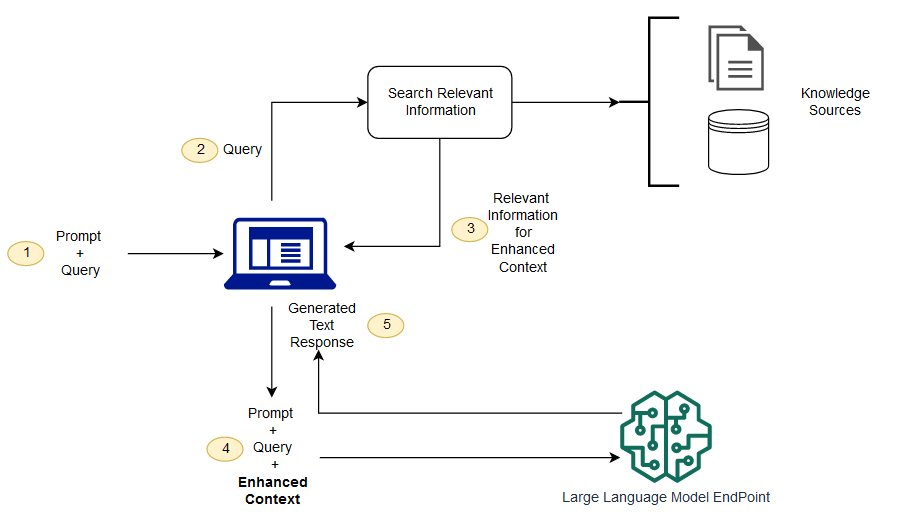
\includegraphics[width=0.80\textwidth]{Images/Cosolythuyet/flow-of-using-rag-with-llms.jpg}
    \caption{Luồng sử dụng RAG với mô hình ngôn ngữ lớn (nguồn: AWS, 2024)\parencite{aws2024genai}.}
    \label{fig:rag_llm_flow}
\end{figure}

Bộ nhớ hội thoại lưu các tiêu chí đang có hiệu lực, sản phẩm được tham chiếu và quyết
định đã xác nhận. Có thể kết hợp lịch sử gần nhất, bản tóm tắt và trạng thái có cấu trúc
để xử lý các câu rút gọn như ``đổi sang màu đen''. Bộ nhớ phải được phân tách theo người
dùng và phiên, đồng thời có giới hạn dung lượng và thời gian lưu trữ.

Một trạng thái có cấu trúc tối thiểu nên có các trường
\texttt{active\_constraints}, \texttt{referenced\_products}, \texttt{last\_intent},
\texttt{pending\_action} và \texttt{confirmed\_facts}. Mỗi lượt, hệ thống chỉ đưa vào
prompt những trường còn hiệu lực; thông tin hết hạn hoặc chưa được xác nhận không được
dùng làm ràng buộc. Sau khi LLM sinh câu trả lời, Backend kiểm tra các mã sản phẩm,
giá, tồn kho và trạng thái đơn trong context trước khi hiển thị, tạo giỏ hàng hoặc
thực hiện thao tác giao dịch.

\subsection{Cơ sở đánh giá hệ thống}
\label{sec:evaluation-foundations}

Với kết quả top-$k$, Hit@$k$ cho biết có ít nhất một sản phẩm liên quan; Precision@$k$
đo tỷ lệ kết quả liên quan; Recall@$k$ đo mức bao phủ; MRR phản ánh vị trí kết quả đúng
đầu tiên; còn nDCG@$k$ xét cả mức độ liên quan và thứ hạng
\parencite{manning2008irbook,javerlin2002ndcg}. Khi đánh giá tìm kiếm ảnh,
cần phân biệt truy hồi đúng sản phẩm gốc với sản phẩm chỉ tương tự về thị giác.

Gọi $Rel(q)$ là tập sản phẩm liên quan với truy vấn $q$, $R_k(q)$ là tập kết quả đầu
tiên và $rel_i$ là mức liên quan của kết quả ở vị trí $i$, các chỉ số cơ bản được tính bởi
\begin{align}
    Precision@k &= \frac{|Rel(q)\cap R_k(q)|}{k}, &
    Recall@k &= \frac{|Rel(q)\cap R_k(q)|}{|Rel(q)|},\\
    Hit@k(q) &= \mathbf{1}\!\left[Rel(q)\cap R_k(q)\ne\varnothing\right], &
    DCG@k(q) &= \sum_{i=1}^{k}\frac{2^{rel_i}-1}{\log_2(i+1)},\\
    NDCG@k(q) &= \frac{DCG@k(q)}{IDCG@k(q)}.
\end{align}
Trong đó $IDCG@k$ là giá trị DCG@k lý tưởng; lấy trung bình $Hit@k(q)$ trên tập truy
vấn cho biết tỷ lệ truy vấn có ít nhất một kết quả đúng.

Đối với RAG, grounding đo tỷ lệ khẳng định được hỗ trợ bởi context; Context Precision
đánh giá mức liên quan của các mục được truy hồi và Context Recall đo mức bao phủ dữ
kiện cần thiết; đây là các chiều đánh giá được đề xuất cho pipeline RAG
\parencite{es2024ragas}. Có thể bổ sung Success Rate cho tỷ lệ hoàn thành tác vụ và tỷ lệ đáp ứng
đồng thời mọi ràng buộc cứng.

Độ trễ nên được báo cáo theo p50, p95 và p99 thay vì chỉ dùng trung bình; ngoài latency
end-to-end, nên tách thời gian hiểu truy vấn, embedding, truy vấn vector, reranking, đọc
dữ liệu nghiệp vụ và sinh phản hồi để cân bằng chất lượng, độ trễ và chi phí.

Với $n$ lần đo độ trễ $t_1,\ldots,t_n$, percentile mức $\alpha$ có thể định nghĩa bởi
\begin{equation}
    p_{\alpha}=\inf\left\{x:\frac{1}{n}\sum_{i=1}^{n}
    \mathbf{1}[t_i\le x]\ge\alpha\right\}.
    \label{eq:latency_percentile}
\end{equation}
Do đó p95 và p99 lần lượt lấy $\alpha=0{,}95$ và $\alpha=0{,}99$. Cần ghi rõ trạng thái
cache và kích thước candidate pool để kết quả giữa các cấu hình có thể tái lập.

\medskip\noindent\textbf{Kết chương.}
Chương đã trình bày nền tảng về embedding, truy hồi vector, lọc ràng buộc, Hybrid Search
image-conditioned, LLM--RAG và phương pháp đánh giá. Trên cơ sở đó, đề tài tách truy
hồi văn bản khỏi truy hồi hình ảnh, dùng metadata kiểm soát ràng buộc, ưu tiên độ tương
tự ảnh cho truy vấn image-conditioned và giới hạn LLM ở việc hiểu truy vấn, tạo phản
hồi có căn cứ, làm nền tảng cho các chương công nghệ, thiết kế và kiểm thử.
